\section{Proportional Integral Derivative Controller}\label{design:PID}
The following section will be based on \cite{PIDcontrolsystem}. In this project the proportional-integral-derivative (PID) controller will be used to make the motors more precise and able to move to a specific amount of degrees, something the motors were found to be incapable of themselves as seen in \cref{sec:actuators}. A PID controller is a commonly used control system. It can be used on a variety of systems and is popular, partly because of its robustness and simplicity, but also because it can be used in many systems with only minor changes. A PID controller is based on a control feedback loop, where the first execution of the loop only uses the current state and the goal state in the calculations. Subsequent executions of the loop uses information about the effects the previous loops had on the system.

\subsection{PID Structure}
A PID controller uses the terms \emph{P}, \emph{I} and \emph{D}, which summed up gives the change that will be applied to the actuator. \emph{P} is the proportional term, \emph{I} is the integral term and \emph{D} is the derivative term. The controller takes two inputs: the target state and the current state. The target state is the state that the PID controller is trying to reach, while the current state is the state the system is currently in. A PID controller has three coefficients: $K_p$, $K_i$, $K_d$ and two variables: \emph{lasterror} and \emph{integral}. The coefficients are part of the three terms and determine their effect on the system. An \emph{error}, see \cref{pidpseudo1}, is a number representing the difference between the current state and the target state. All errors are continuously summed up and stored in \emph{integral}. \emph{lasterror} is the error from the last state to the current state. The bigger the \emph{error} is, the more the system has to correct to reach the target state. The \emph{error} influences all the terms. \\

\emph{Proportional} is the error as it is in the current state, and it is used to make the system move towards the target. $K_p$ determines the magnitude of this term. \\

\emph{Integral} is the sum of all errors, and it increases continuously as long as the target state is not reached. Both \emph{P} and \emph{D} can reach zero if the error is sufficiently small, this problem is called steady-state error. In case of a steady-state error \emph{I} will continue to grow and will eventually start changing the system. The magnitude of the \emph{integral} term is decided by the size of $K_i$.\\

\emph{Derivative} is the difference in the error between the current state and last state, divided by the time since the last state. It is used to stabilize the system faster, as it attempts to predict the future. The magnitude of the derivative term is decided by the size of $K_d$. 


\begin{lstlisting}[style=customc, label={pidpseudo1}, caption={Pseudo code of a PID controller}]
//K_p, K_i and K_D are the PID coefficients that have been predefined
lasterror = 0
integrale = 0
PID(target, current)
    error = target - current
    integrale = integrale + error
    derivative = lasterror - error
    lasterror = error

    return Kp * error + Ki * integrale + Kd * derivative
\end{lstlisting}

\Cref{pidpseudo1} is working in the discrete time space and therefore $\Delta t$ is used in \emph{Integral} and \emph{Derivative}. In order to save calculations, $\Delta t$ has been integrated into the coefficients, this can be done as $\Delta t$ was chosen to be static.

\subsection{PID Tuning}
In order to make the PID controller work properly the three coefficients need to be tuned. There are several methods available for PID tuning, however, only two will be described here: manual tuning and the Ziegler-Nichols method. The Ziegler-Nichols method was chosen as it is a mathematically proven method~\cite{Ziegler-Nichols}, and manual tuning because it is a good way to make changes to the PID controller based on specific demands. Because these two methods are sufficient, other methods will not be explored.

\begin{table}[H]
\centering
\begin{tabular}{|l|l|l|l|}
\hline
\textbf{Control Type} & \textbf{$K_p$}     & \textbf{$K_i$}        & \textbf{$K_d$}      \\ \hline
P            & $0.50K_u$ & -            & -          \\ \hline
PI           & $0.45K_u$ & $1.2K_p/T_u$ & -          \\ \hline
PID          & $0.60K_u$ & $2K_p/T_u$   & $K_pT_u/8$ \\ \hline
\end{tabular}
\caption{Ziegler-Nichols Method}
\label{Ziegler-Nichols_Method}
\end{table}

The Ziegler-Nichols method is well defined and it is used to tune a PID controller. The first step of the method is to set $K_i$ and $K_d$ to zero. $K_p$ is then slowly increased until the motor oscillates. $T_u$ is the rate at which it oscillates, and $K_u$ is the $K_p$ value at which it oscillates. The three PID controller terms can then be calculated as shown in \cref{Ziegler-Nichols_Method}. This way of tuning is aggressive and will result in a fast rise, it might even result in some overshoot.

\begin{table}[H]
\centering
\small
\begin{tabular}{|l|l|l|l|l|l|}
\hline
           & \textbf{Rise time}    & \textbf{Overshoot} & \textbf{Settling time} & \textbf{Steady-state error}  & \textbf{Stability}              \\ \hline
$K_p$      & Decrease     & Increase  & Small change  & Decrease            & Degrade                \\ \hline
$K_i$      & Decrease     & Increase  & Increase      & Eliminate           & Degrade                \\ \hline
$K_d$      & Minor change & Decrease  & Decrease      & No effect in theory & Improve if $K_d$ small \\ \hline
\end{tabular}
\caption{Impact of increasing a parameter \cite{PIDcontrolsystem}.}
\label{Manual-tuning}
\end{table}
\FloatBarrier

Another method of system tuning is manual tuning. To use this method it is necessary to know which effect changing the coefficients has on the system. This information can be gathered from a tuning table, such as \cref{Manual-tuning}, and then the coefficients can be tuned through a trial-and-error approach or meta optimization \cite{PIDmetaOptimization}. \Cref{pidsettling} shows a graph containing the properties of a PID controller. The rise time is the time it takes for a PID controller to reach the target state for the first time, a short rise time tends to result in overshoot. Overshoot is how much a PID controller misses the target by the first time, in some systems overshoot may be prohibited. The settling time is how long it takes to reach a steady state. There might be a steady state error when there is a small error when the steady state is reached. A PID controller can be unstable and never reach a steady state which means that the coefficients have to be changed in order to stabilize the system.

\begin{figure}[H]
\centering
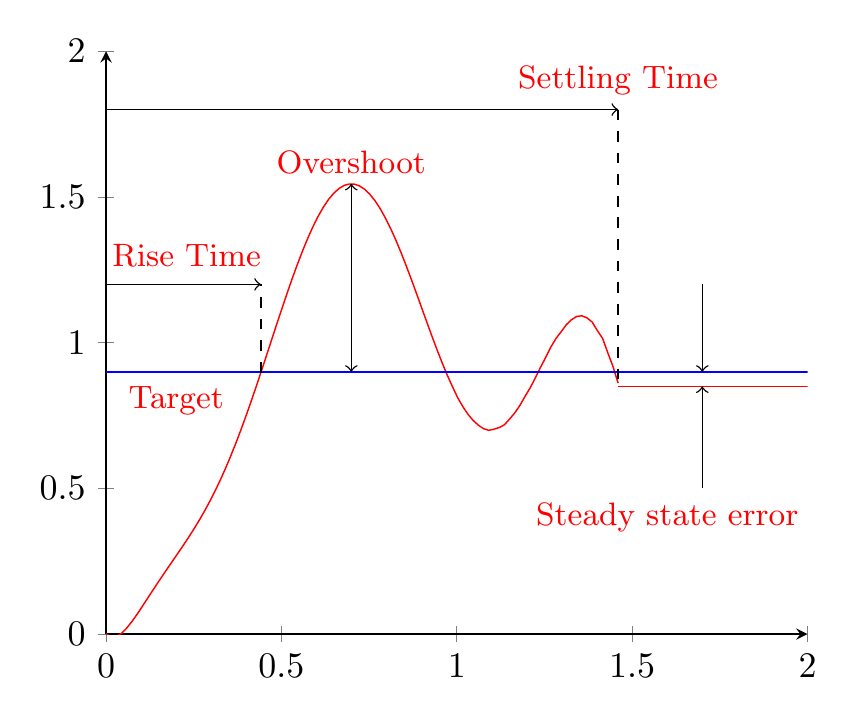
\begin{tikzpicture}[scale=1.3]
\begin{axis}[
    axis lines = left,
    xmin=0,xmax=2,
    ymin=0,ymax=2,
]

%Below the red parabola is defined
\addplot [
    domain=0:1.46, 
    samples=100, 
    color=red,
]
{80.83892322*x^8-473.66979127*x^7+1095.0629877*x^6-1265.55113227*x^5+768.48166718*x^4-242.51503181*x^3+39.47160828*x^2-1.30063244*x+0.00131008};

\addplot[color=red, domain=1.46:2] coordinates {
		(1.4598,0.85)
		(2,0.85)
};
\addplot[color=blue, domain=0:2] coordinates {
		(0,0.9)
		(2,0.9)
};
\addplot[<->,color=black, domain=0:2] coordinates {
		(0.69925398,1.5451)
		(0.69925398,0.9)
};

\node[red] at (axis cs:0.69925398,1.62){\small{Overshoot}};

\addplot[->,color=black, domain=0:2] coordinates {
        (1.7,1.2)
		(1.7,0.9)
};
\addplot[->,color=black, domain=0:2] coordinates {
        (1.7,0.5)
		(1.7,0.85)
};
\node[red] at (axis cs:1.6,0.4){\small{Steady state error}};

\addplot[color=black, domain=0:2, dashed] coordinates {
		(0.4415,0.8976)
		(0.4415,1.2)
};
\addplot[->,color=black, domain=0:2] coordinates {
		(0,1.2)
		(0.4415,1.2)
};
\node[red] at (axis cs:0.23,1.3){\small{Rise Time}};

\addplot[color=black, domain=0:2, dashed] coordinates {
		(1.4598,1.8)
		(1.4598,0.85)
};

\addplot[<-,color=black, domain=0:2] coordinates {
		(1.4598,1.8)
		(0,1.8)
};

\node[red] at (axis cs:0.2,0.8){\small{Target}};

\node[red] at (axis cs:1.4598,1.9){\small{Settling Time}};
\end{axis}
\end{tikzpicture}
\caption{PID properties.}\label{pidsettling}
\end{figure}

\subsection{PID Usage}
As the motors can only be controlled by setting a power percentage the PID controller was be used as an extra control layer. The PID controller is tuned by first using the Ziegler-Nichols method to create a stable system. Once a stable system has been found it will be fine tuned to avoid overshoot by using manual tuning. By lowering $K_p$ and $K_i$ the overshoot will decrease while the rise time increases. A compromise where to be found where the overshoot is small and the rise time is not too long.

